\documentclass{article}
\usepackage[utf8]{inputenc}
\usepackage{listings}
\usepackage{xcolor}
\usepackage{subcaption}
\usepackage{minted}

\definecolor{codegreen}{rgb}{0,0.6,0}
\definecolor{codegray}{rgb}{0.5,0.5,0.5}
\definecolor{codepurple}{rgb}{0.58,0,0.82}
\definecolor{backcolour}{rgb}{0.95,0.95,0.92}
\usepackage{color}   %May be necessary if you want to color links
\usepackage{hyperref}
\usepackage{graphicx}
\hypersetup{
    colorlinks=true, %set true if you want colored links
    linktoc=all,     %set to all if you want both sections and subsections linked
    linkcolor=black,  %choose some color if you want links to stand out
    urlcolor=blue,
}
\lstdefinestyle{mystyle}{
    backgroundcolor=\color{backcolour},   
    commentstyle=\color{codegreen},
    keywordstyle=\color{magenta},
    numberstyle=\tiny\color{codegray},
    stringstyle=\color{codepurple},
    basicstyle=\ttfamily\footnotesize,
    breakatwhitespace=false,         
    breaklines=true,                 
    captionpos=b,                    
    keepspaces=true,                 
    numbers=left,                    
    numbersep=5pt,                  
    showspaces=false,                
    showstringspaces=false,
    showtabs=false,                  
    tabsize=2
}

\lstset{style=mystyle}


\title{SMBUD}
\author{Filippo Lazzati, Martina Magliani, Christian Grasso, Sofia Martellozzo, Giacomo Lombardo}
%\date{October 2021}

\begin{document}
\thispagestyle{empty}
\begin{titlepage}
    \begin{center}
       %\vspace*{2cm}
       {\Huge \textbf{SMBUD}} %%Replace this with the Title of your research
       \vspace{0.5cm}
       \\
    \begin{LARGE}
        {Vaccinations Analysis}
        \vspace{1.0cm}
        \\
        {\textit{Specification, data model and Elasticsearch analysis}}
           
\includegraphics[width=13cm]{logo/polimi.png}
          \vspace{1.5cm}\\
                  Filippo Lazzati (10629918) - Martina Magliani (10682333) - Christian Grasso (10652464) - Sofia Martellozzo (10623060) - Giacomo Lombardo (10674987)\\
       {Year: 2021/2022}
    \end{LARGE}  
   \end{center}
\end{titlepage}
\newpage
\tableofcontents %this command creates an index
\newpage
\section{Problem specification}
The purpose of this project is to design, store and query data on a NoSQL database in order to analyze data about COVID-19 vaccination statistics.\\ Starting from an open \href{https://raw.githubusercontent.com/italia/covid19-opendata-vaccini/master/dati/somministrazioni-vaccini-latest.csv}{dataset} containing raw data about the distribution and administration of COVID-19 vaccines in Italian regions, the main goal of the project is to obtain relevant information through queries and graphs.\\
To perform this task, the dataset has been loaded into \textbf{ElasticSearch}, a search engine with an internal database focused on high performances that interacts with external components through RESTful APIs. Once loaded into the search engine, information can be retrieved from the dataset not only through queries but also through Kibana, a powerful user interface that allows to visualize ElasticSearch data. More specifically, through \textbf{Kibana} it is possible to create Dashboards that generate and display graphs and other significant information in an intuitive way.\\
\subsection{Dataset}
The used dataset is provided by the Italian Government and contains the official data about vaccines distribution and administration. More specifically it provides regional overview of the amount of doses administered every day in the time period between 27/12/2020 and today.
The dataset contains 15 fields, which are briefly summarized in the following:
\begin{itemize}
    \item \textbf{index}, a unique identifier of the record;
    \item \textbf{area}, an acronym of the region at issue;
    \item \textbf{fornitore}, the brand provider of the vaccine; 
    \item \textbf{data\_somministrazione}, the date when the vaccine doses have been administered;
    \item \textbf{fascia\_anagrafica}, the age range the people who received the vaccination belong to;
    \item \textbf{sesso\_maschile}, the number of males vaccinated;
    \item \textbf{sesso\_femminile}, the number of females vaccinated;
    \item \textbf{prima\_dose}, the number of first doses;
    \item \textbf{seconda\_dose}, the number of second doses;
    \item \textbf{pregressa\_infezione}, the number of doses administered to people who came down with the disease between 3 and 6 months ago;
    \item \textbf{dose\_addizionale\_booster}, the number of third doses admininstered;
    \item \textbf{codice\_NUTS1}, European classification of NUTS level 1;
    \item \textbf{codice\_NUTS2}, European classification of NUTS level 2;
    \item \textbf{codice\_regione\_ISTAT}, ISTAT code of the region;
    \item \textbf{nome\_regione}, the name of the region.
\end{itemize}
The way this dataset has been imported into \verb|ElasticSearch| is shown in section \ref{Conceptual model}.\\
According to the project's specifications, the possibility of integrating the project with an additional dataset is contemplated. Therefore, we have decided to add a secondary dataset,\href{https://github.com/italia/covid19-opendata-vaccini/blob/master/dati/consegne-vaccini-latest.csv}{consegne-vaccini-latest}, that contains additional information about the amount of daily delivered doses in the same time period, to better contextualise the primary dataset. Such secondary dataset contains 8 field, briefly explained in the following:
\begin{itemize}
    \item \textbf{index}, a unique identifier of the record;
    \item \textbf{area}, an acronym of the region at issue;
    \item \textbf{fornitore}, the brand provider of the vaccine; 
    \item \textbf{data\_consegna}, the date when the vaccine doses have been delivered;
    \item \textbf{numero\_dosi}, the number of doses delivered;
    \item \textbf{codice\_NUTS1}, European classification of NUTS level 1;
    \item \textbf{codice\_NUTS2}, European classification of NUTS level 2;
    \item \textbf{codice\_regione\_ISTAT}, ISTAT code of the region;
    \item \textbf{nome\_regione}, the name of the region.
\end{itemize}
\newpage

%---------------------------------%
\section{Conceptual model}\label{Conceptual model}
In \verb|ElasticSearch|, there are two ways to create a schema (model) of the data we are importing in the database. We have to remember that \verb|ElasticSearch| is an Information Retrieval system that contains an inner document-oriented database, which means that we can store data at the granularity level of documents, the same of \verb|MongoDB|. In the \verb|ElasticSearch| world, the schema of the data is called \textit{mapping}, and can be of two types:
\begin{itemize}
    \item \href{https://www.elastic.co/guide/en/elasticsearch/reference/current/dynamic-mapping.html}{dynamic mapping}, which is automatically carried out by \verb|ElasticSearch|, which autonomously tries to infer the datatypes of the fields;
    \item \href{https://www.elastic.co/guide/en/elasticsearch/reference/current/explicit-mapping.html}{explicit mapping}, in which we have to explicitly define the type of the fields when creating an index\footnote{In the \verb|ElasticSearch| world, an index can be seen as a table of RDBS.}.
\end{itemize}
It is clear that dynamic mapping can fail, therefore we have to be cautious when using it.\\
In our project, we have decided to exploit dynamic mapping because the mapping inferred perfectly coincides with the one we would have defined. In fact, you can notice this in the following json code, which is provided by \verb|ElasticSearch| to justify the dynamic mapping:
\begin{minted}{json}
{
  "properties": {
    "@timestamp": {
      "type": "date"
    },
    "area": {
      "type": "keyword"
    },
    "codice_NUTS1": {
      "type": "keyword"
    },
    "codice_NUTS2": {
      "type": "keyword"
    },
    "codice_regione_ISTAT": {
      "type": "long"
    },
    "data_somministrazione": {
      "type": "date",
      "format": "iso8601"
    },
    "dose_addizionale_booster": {
      "type": "long"
    },
    "fascia_anagrafica": {
      "type": "keyword"
    },
    "fornitore": {
      "type": "keyword"
    },
    "nome_area": {
      "type": "keyword"
    },
    "pregressa_infezione": {
      "type": "long"
    },
    "prima_dose": {
      "type": "long"
    },
    "seconda_dose": {
      "type": "long"
    },
    "sesso_femminile": {
      "type": "long"
    },
    "sesso_maschile": {
      "type": "long"
    }
  }
}
\end{minted}
The mapping requires some observations:
\begin{itemize}
    \item the type \textbf{keyword} is used for structured content such as IDs, email addresses, hostnames, status codes, zip codes, or tags, therefore it perfectly fits for codes like "codice\_NUTS1", or "area", or "fornitore", ... etc.; notice that it is ok for us also to have "fascia\_anagrafica" as \textbf{keyword}, since we do not need to perform text search on it;
    \item the type \textbf{long} is a numeric datatype that represents a signed 64-bit integer with a minimum value of $-2^{63}$ and a maximum value of $2{63}-1$; basically, it is type \textbf{integer} but enlarged with more bytes, therefore it is suited for all the numeric values we have in the dataset;
    \item the only date field, "data\_somministrazione", has been properly inferred as a date, thanks to the fact that it was encoded in the standard format iso8601;
    \item it is better to spend some words about field "area". As a matter of fact, it has been inferred of type "keyword", which is ok for our purposes; however, it can be matched 1-to-1 to a region of Italy, therefore in order to provide a map view in the \verb|Kibana| dashboard, later on we have provided some rows of explanation about how to match field "area" to "geo\_shape" datatype, which allows to draw it as a polygon.
\end{itemize}

As far as the second dataset is concerned, there are few differences with what previously stated:
\begin{minted}{json}
{
  "properties": {
    "@timestamp": {
      "type": "date"
    },
    "area": {
      "type": "keyword"
    },
    "codice_NUTS1": {
      "type": "keyword"
    },
    "codice_NUTS2": {
      "type": "keyword"
    },
    "codice_regione_ISTAT": {
      "type": "long"
    },
    "data_consegna": {
      "type": "date",
      "format": "iso8601"
    },
    "fornitore": {
      "type": "keyword"
    },
    "nome_area": {
      "type": "keyword"
    },
    "numero_dosi": {
      "type": "long"
    }
  }
}
\end{minted}
As it can be easily seen by the json provided, the date "data\_consegna" has been properly inferred, as well as all the other fields, therefore we can easily adopt dynamic mapping also for this dataset.
\newpage
%---------------------------------%
\section{Queries and Commands}
In this section we present some queries and some commands that we consider useful to manage the considered data. It should be remarked that we can interact with \verb|ElasticSearch| through REST APIs, since it is RESTful, and that there are various ways to interfacing with it; the most used are:
\begin{itemize}
\item a REST client application like \href{https://www.postman.com}{Postman};
    \item a client like \href{https://curl.se
}{curl};
\item \verb|Kibana|, the graphical user interface of \verb|ElasticSearch|. This is the way we adopt.
\end{itemize}
You have to notice also that you have to upload the datasets with names "somministrazioni-vaccini-latest" and "consegne-vaccini-latest" in order to use the following queries and commands.
\subsection{Queries}
We have identified the following queries:
\begin{enumerate}
\item \textbf{find the number of vaccines administered by brand in the last 30 days and also the brand with the highest number}.\\
In order to perform this query, we have to use the \verb|GET| method (like all the other queries). Moreover, we have to filter the results through "query" to retrieve data that is not older than 30 days and then we have to exploit a script to sum the values of fields "sesso\_maschile" and "sesso\_femminile". Then, we have to aggregate by brand ("fornitore") to compute meaningful sums. Finally, to retrieve the brand with the highest number of vaccines administered we have to exploit also the "max\_bucket" construct:
\begin{lstlisting}
GET /somministrazioni-vaccini-latest/_search
{
  "size": 0,
  "query": {
    "range": {
      "@timestamp": {
        "gte": "now-30d/d",
        "lt": "now/d"
      }
    }
  },
  "runtime_mappings": {
    "vaccini": {
      "type": "long",
      "script": """
        long total = doc['sesso_maschile'].value + doc['sesso_femminile'].value;
        emit(total);
      """
    }
  },
  "aggs": {
    "vaccinations_per_brand": {
      "terms": {
        "field": "fornitore"
      },
      "aggs": {
        "total_vaccinations": {
          "sum": {
            "field": "vaccini"
          }
        }
      }
    }
  ,
    "most-used_brand": {
      "max_bucket": {
        "buckets_path": "vaccinations_per_brand > total_vaccinations" 
      }
  }
}
}
\end{lstlisting}
\item \textbf{find the region with the highest number of first vaccinations in the last 3 months}.\\
The query is similar to the previous one. We have to filter the results by date through "query", and then exploit nested "aggs" to compute the sum of field "prima\_dose" aggregated by region; finally we draw the maximum in the same way as before:
\begin{lstlisting}
GET /somministrazioni-vaccini-latest/_search
{
  "size": 0,
  "query": {
    "range": {
      "@timestamp": {
        "gte": "now-90d/d",
        "lt": "now/d"
      }
    }
  },
  "aggs": {
    "first_vaccinations_per_region": {
      "terms": {
        "field": "area"
      },
"aggs": {
        "first_vaccinations": {
          "sum": {
            "field": "prima_dose"
          }
        }
}
  },
    "most-vaccinated_region": {
      "max_bucket": {
        "buckets_path": "first_vaccinations_per_region > first_vaccinations" 
      }
  }
}
}

\end{lstlisting}
\item \textbf{find the total number of boosters in Italy in last 30 days}.\\
This query is quite easy; indeed, we have to filter the results by date and then return the sum of field "dose\_addizionale\_booster":
\begin{lstlisting}
GET /somministrazioni-vaccini-latest/_search
{
  "size": 0,
  "query": {
    "range": {
      "@timestamp": {
        "gte": "now-30d/d",
        "lt": "now/d"
      }
    }
  },
  "aggs": {
    "total_number_of_boosters": {
      "sum": {
        "field": "dose_addizionale_booster"
      }
  }
  }
}
\end{lstlisting}
\item \textbf{find the age range with the highest number of vaccinations in the last 30 days.}
The pattern is similar to the first query; namely, we use a script after having filtered the results by date to compute the sum of male and female vaccine doses and finally we return the maximum value:
\begin{lstlisting}
GET /somministrazioni-vaccini-latest/_search
{
  "size": 0,
  "query": {
    "range": {
      "@timestamp": {
        "gte": "now-30d/d",
        "lt": "now/d"
      }
    }
  },
  "runtime_mappings": {
    "vaccini": {
      "type": "long",
      "script": """
        long total = doc['sesso_maschile'].value + doc['sesso_femminile'].value;
        emit(total);
      """
    }
  },
  "aggs": {
    "vaccinations_per_age_range": {
      "terms": {
        "field": "fascia_anagrafica"
      },
      "aggs": {
        "total_vaccinations": {
          "sum": {
            "field": "vaccini"
          }
        }
      }
    }
  ,
    "most-used_brand": {
      "max_bucket": {
        "buckets_path": "vaccinations_per_age_range > total_vaccinations" 
      }
  }
}
}
\end{lstlisting}
\item \textbf{find the total number of Moderna doses received in the last 3 days in Italy}.\\
We simply have to filter the data both by "fornitore" and date before computing the sum of field "numero\_dosi":
\begin{lstlisting}
GET /consegne-vaccini-latest/_search
{
  "size": 0,
  "query": {
    "bool": {
      "filter": [
        {"term": {
          "fornitore": "Moderna"
        }
        },
        {"range": {
      "@timestamp": {
        "gte": "now-3d/d",
        "lt": "now-1d/d"
      }
     }
    }
  ]
    }},
  "aggs": {
    "vaccine_doses_received": {
      "sum": {
        "field": "numero_dosi"
      }
    }
  }
}
\end{lstlisting}
\item \textbf{find the region with the highest disparity of vaccinations between males and females}.\\
This query is more tricky than the previous one because it involves a script in which we have to compute the absolute value of a difference (we do not know whether there are more males that undergo vaccination or females, and we do not want to return negative values). The rest of the query is similar to the others:
\begin{lstlisting}
GET /somministrazioni-vaccini-latest/_search
{
  "size": 0,
    "runtime_mappings": {
      "vaccini": {
        "type": "long",
        "script": """
          long total = doc['sesso_maschile'].value - doc['sesso_femminile'].value;
          if(total < 0){
            total = total * - 1;
          }
          emit(total);
      """
    }},
    "aggs": {
      "vaccinations_per_region":{
      "terms": {
          "field": "nome_area"
        },
        "aggs": {
        "max_dif_of_vaccinations_between_male_female": {
          "max": {
            "field": "vaccini"
          }
     }
          
        }},
      "highest_disparity_of_vaccinations": {
        "max_bucket": {
          "buckets_path": "vaccinations_per_region > max_dif_of_vaccinations_between_male_female" 
     }
    }
  }
}
\end{lstlisting}
\item \textbf{number of children between 5-11 vaccinated this week in Basilicata}.\\
DOES NOT WORK
\begin{lstlisting}
   GET /somministrazioni-vaccini-latest/_count
{
  "query": {
    "bool": {
      "must": [
	{ "match" : 
	    "fascia_anagrafica": "5-11" 
	},
        { "range" : {
	    "@timestamp": {
		"gte": "now-7d/d",
		"lte": "now/d"
	    }
        },
        { "match" : {
            "nome_area": "Basilicata"
        }
      ]
    }
  }
}
\end{lstlisting}
\item \textbf{to do}.\\
DOES NOT WORK
\begin{lstlisting}
   
\end{lstlisting}
\item \textbf{brand of the less-used vaccine with young people (<30 years old)}.\\
DOES NOT WORK
\begin{lstlisting}
GET /somministrazioni-vaccini-latest/_search
{
  "query": {
    "bool": {
      "should": [
	{ "match" : 
	    "fascia_anagrafica": "5-11" 
	},
	{ "match" : 
	    "fascia_anagrafica": "12-19" 
	},
        { "match" : 
	    "fascia_anagrafica": "20-29" 
	}
      ]
   },
    "runtime_mappings": {
    "vaccini": {
      "type": "long",
      "script": """
        long total = doc['sesso_maschile'].value + doc['sesso_femminile'].value;
        emit(total);
      """
    }
   },
   "aggs": {
    "vaccinations_per_region": {
      "terms": {
        "field": "nome_area"
     },
      "aggs": {
        "total_vaccinations": {
          "sum": {
            "field": "vaccini"
          }
     },
      "less-used_brand": {
        "min_bucket": {
          "buckets_path": "vaccinations_per_region > total_vaccinations" 
     }
  }
}
\end{lstlisting}
\end{enumerate}
\subsection{Commands}
We have identified the following commands to show how the system works:\\
\begin{enumerate}
    \item \textbf{Update one specific document (data of Abruzzo 2020/03/30 for age range 40-49 for Moderna) with specific data (100 males vaccinated and 2012 second doses)}.\\
    The construct we use is the "\_update\_by\_query" one, which can be used with the \verb|POST| method; we have to perform a query to find the document to update, and then we exploit a script (with parameters) to update the document:
\begin{lstlisting}
        POST /somministrazioni-vaccini-latest/_update_by_query
{
  "query": {
    "bool": {
      "filter": [
        {"term": {"area": "ABR"}},
        {"term": {"fascia_anagrafica": "40-49"}},
        {"term": {"fornitore": "Moderna"}},
        {
          "range": {
            "@timestamp": {
              "time_zone": "+02:00",
              "gte": "2020-03-30T00:00:00",
              "lt": "2020-03-31T00:00:00"
            }
          }
        }
      ]
    }
  },
  "script": {
    "source": "ctx.sesso_maschile = params.sesso_maschile; ctx.seconda_dose = params.seconda_dose",
    "lang": "painless",
    "params": {
      "sesso_maschile": 100,
      "seconda_dose": 2012
    }
  }
}
\end{lstlisting}
\item \textbf{Create one new document}.\\
This command is the easiest; we simply have to make a \verb|POST| with "\_doc", and then specify a value for all the fields:
\begin{lstlisting}
        POST /somministrazioni-vaccini-latest/_doc
{
  "data_somministrazione": "2021-12-28",
  "fornitore": "Moderna",
  "area": "BAS",
  "fascia_anagrafica": "30-39",
  "sesso_maschile": 910,
  "sesso_femminile": 1211,
  "prima_dose": 93,
  "seconda_dose": 563,
  "pregressa_infezione": 33,
  "dose_addizionale_booster": 1465,
  "codice_NUTS1": "ITF",
  "codice_NUTS2": "ITF5",
  "codice_regione_ISTAT": 17
}
\end{lstlisting}
\end{enumerate}

\section{Kibana Dashboard}
By using the Kibana tool we realised a simple dashboard containing some relevant graphs to visualise the data provided by the dataset.
The dashboard displays the following information and graphs:
\begin{itemize}
    \item total number of administered vaccines;
    \item administered doses of vaccines per region;
    \item administered doses per supplier;
    \item administered doses per week, grouped by:
    \begin{itemize}
        \item supplier;
        \item age range;
        \item gender.
    \end{itemize}
    \item total number of delivered doses;
    \item delivered doses per region;
    \item delivered doses per week.
\end{itemize}



\section{References and sources}
\begin{itemize}
    \item \href{https://www.elastic.co}{Elasticsearch}
    \item \href{https://www.elastic.co/kibana/}{Kibana}
    \item \href{https://github.com/italia/covid19-opendata-vaccini}{Dataset}
    \item \href{https://app.diagrams.net}{draw.io}
\end{itemize}


\section{Image gallery}


\begin{figure}[ht!]
    \centering
    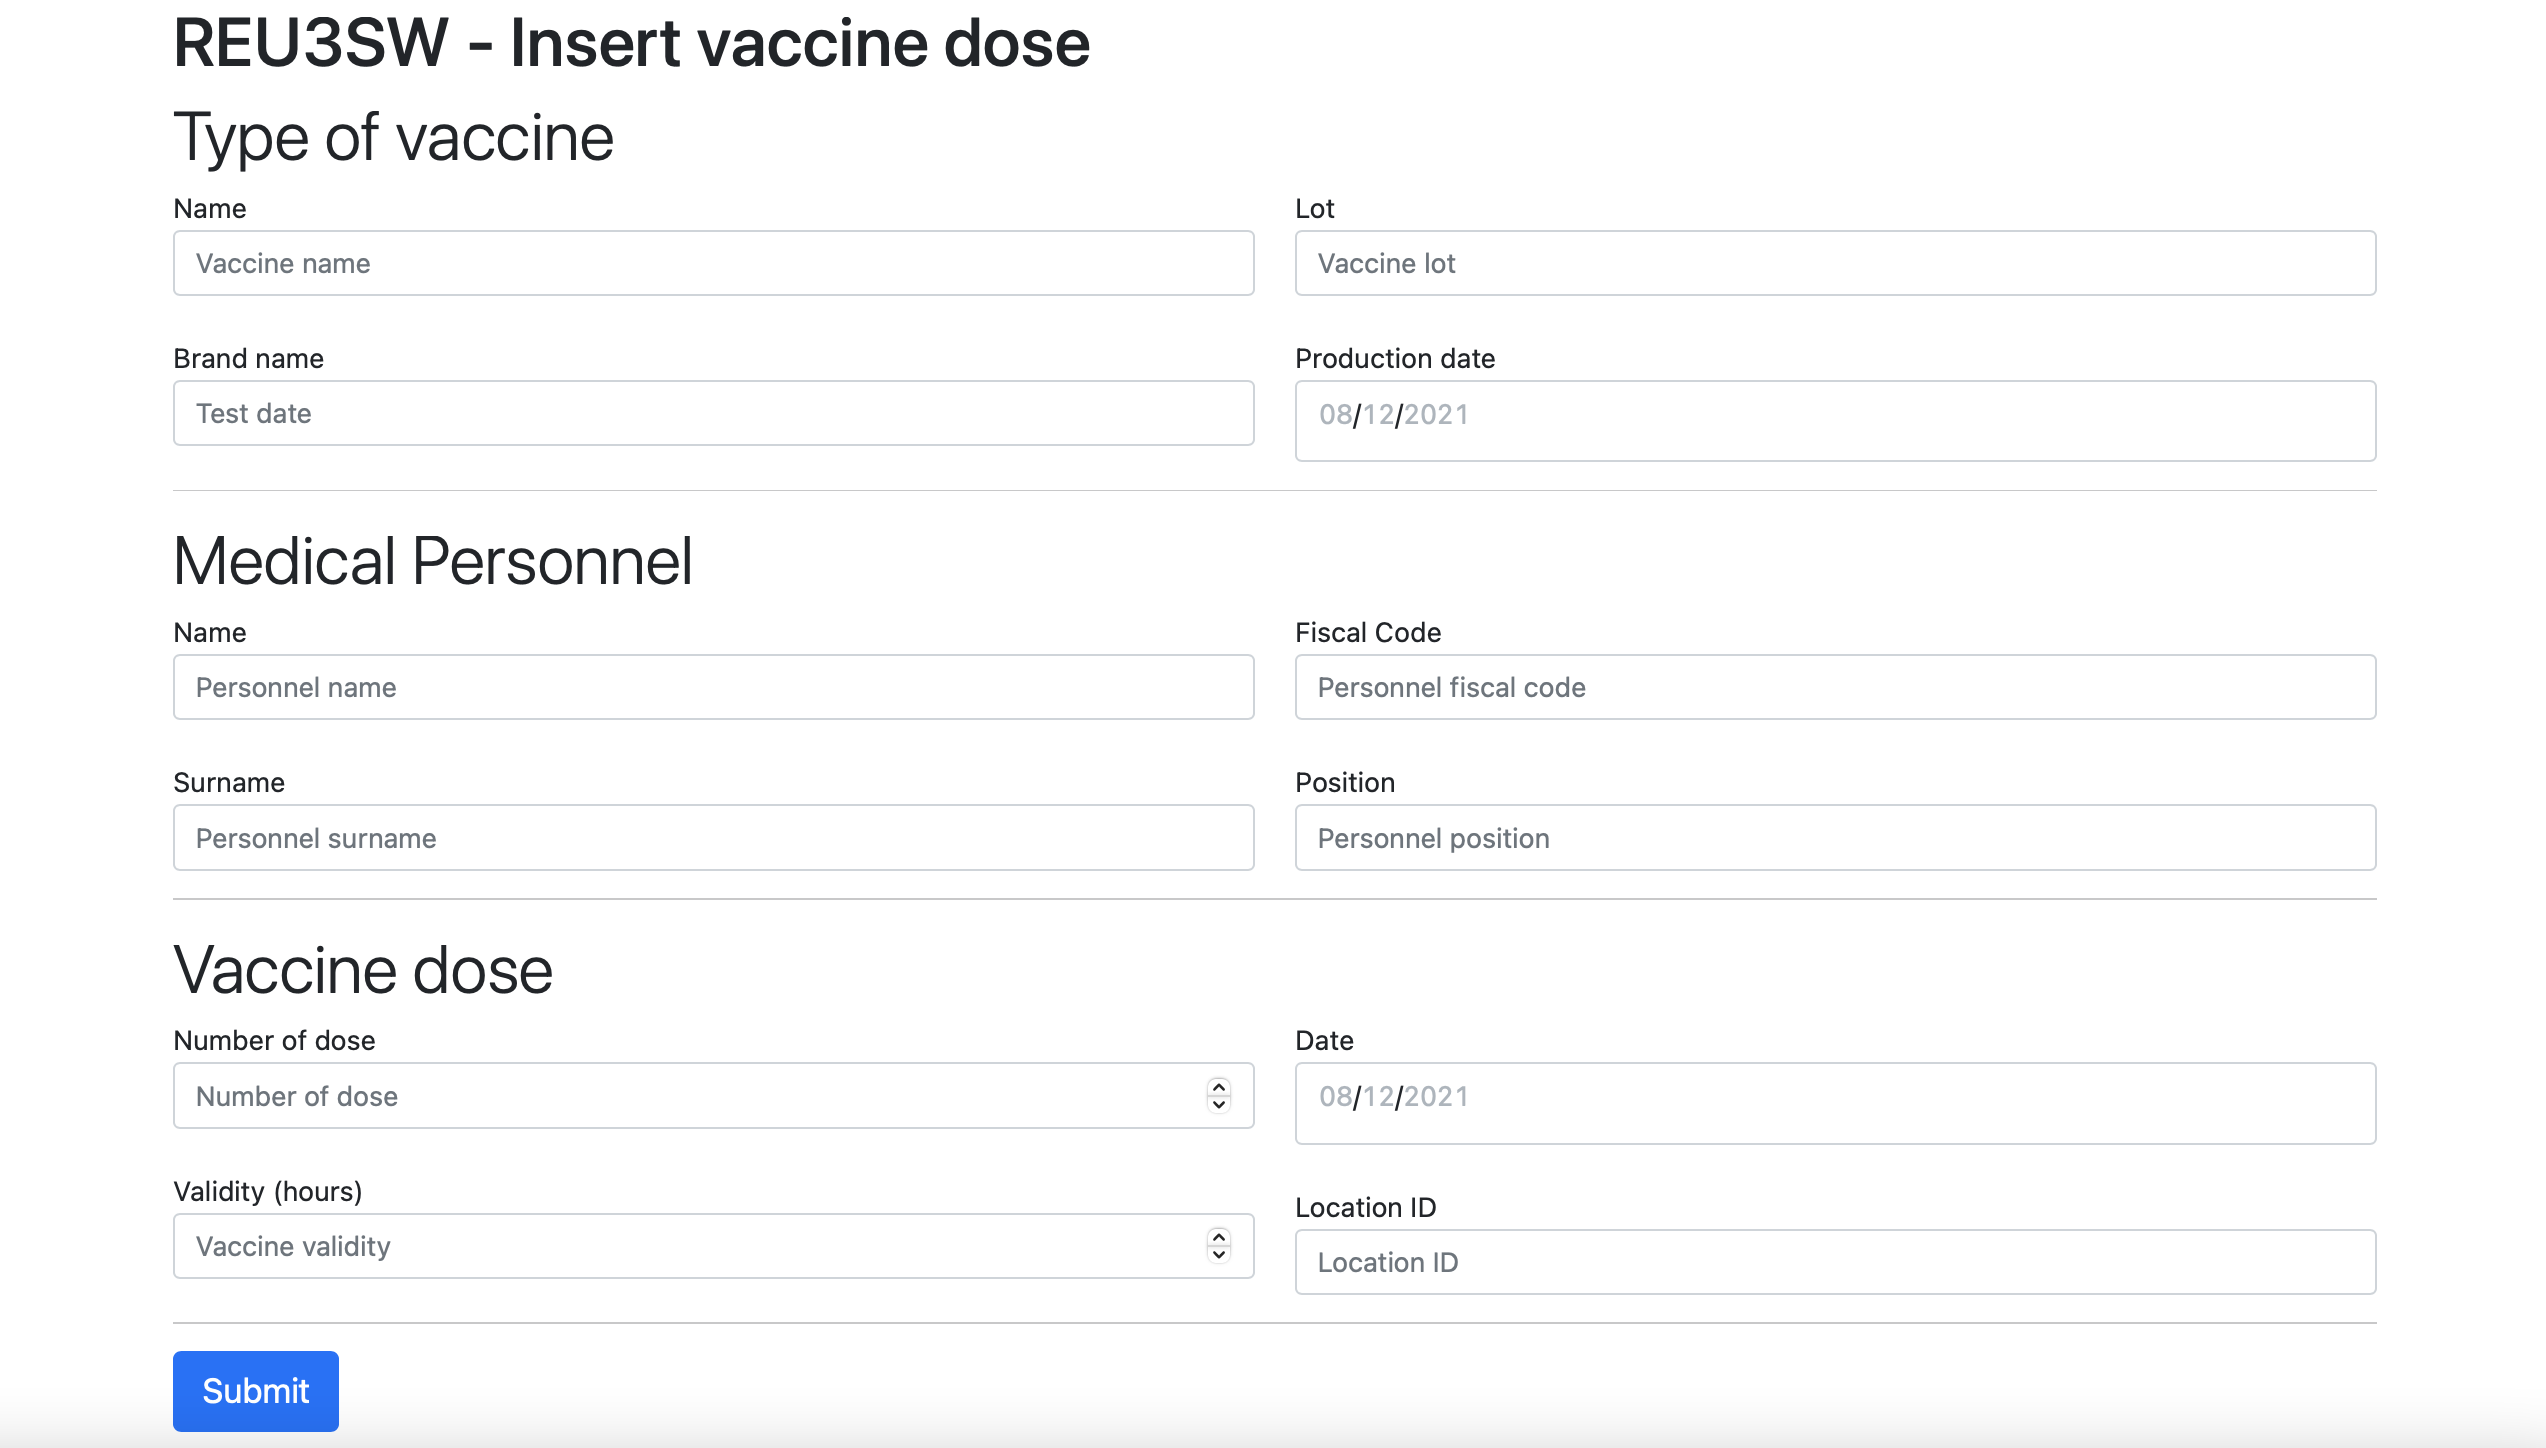
\includegraphics[scale=0.3]{screenshots/insertvaccine.png}
    \caption{Page for the insertion of a new vaccine dose to a person.}
\end{figure}
\end{document}
